





\begin{frame}{Table of Contents}
   \begin{block}{Debugging and Profiling} \end{block}
   \begin{block}{Nonlinear Solvers} \end{block}
   \begin{block}{Unstructured Grids} \end{block}
   \begin{block}{PETSc and GPUs} \end{block}
\end{frame}


%%%%%% General PETSc information %%%%%%%%%%

%
% Why Libraries?
%   - Reinvent the wheel again and again?
%   - Same procedure common for non-software (Theorems, engineering, etc.)
%   - Specialization and settlement of approaches over time (OS, Hardware, etc.)
%   



%
% Debugging and Profiling
%
\section{Debugging and Profiling}
\begin{frame}{PETSc}
   \begin{center} \Large \textbf{Debugging and Profiling} \end{center}
\end{frame}

\subsection{Debugging}
\begin{frame}[fragile]{PETSc Debugging}
  \begin{itemize}
  \item By default, a debug build is provided

  \vspace*{0.3cm}
  \item Launch the debugger
  \begin{itemize}
    \item \lstinline|-start_in_debugger  [gdb,dbx,noxterm]|
    \item \lstinline|-on_error_attach_debugger [gdb,dbx,noxterm]|
  \end{itemize}

  \vspace*{0.3cm}
  \item Attach the debugger only to some parallel processes
  \begin{itemize}
    \item \lstinline|-debugger_nodes 0,1|
  \end{itemize}

  \vspace*{0.3cm}
  \item Set the display (often necessary on a cluster)
  \begin{itemize}
    \item \lstinline|-display :0|
  \end{itemize}
\end{itemize}
\end{frame}  

\begin{frame}{Debugging Tips}

\begin{itemize}
  \item Put a breakpoint in \lstinline|PetscError()| to catch errors as they occur

  \vspace*{0.3cm}
  \item PETSc tracks memory overwrites at both ends of arrays
  \begin{itemize}
    \item The \lstinline|CHKMEMQ| macro causes a check of all allocated memory

    \item Track memory overwrites by bracketing them with \lstinline|CHKMEMQ|
  \end{itemize}

  \vspace*{0.3cm}
  \item PETSc checks for leaked memory
  \begin{itemize}
    \item Use \lstinline|PetscMalloc()| and \lstinline|PetscFree()| for all allocation

    \item Print unfreed memory on \lstinline|PetscFinalize()| with \lstinline|-malloc_dump|
  \end{itemize}

  \vspace*{0.3cm}
  \item Simply the best tool today is {\color{red} Valgrind}
  \begin{itemize}
    \item It checks memory access, cache performance, memory usage, etc.

    \item \href{http://www.valgrind.org}{http://www.valgrind.org}

    \item Pass \lstinline|-malloc 0| to PETSc when running under Valgrind
    \item Might need \lstinline|--trace-children=yes| when running under MPI
    \item \lstinline|--track-origins=yes| handy for uninitialized memory
  \end{itemize}
\end{itemize}

\end{frame}




\begin{frame}[fragile]{PETSc Profiling}

\begin{block}{First: Get the Math Right!}
\begin{itemize}
  \item Choose an algorithm that gives robust iteration counts
  \item Choose an algorithm that really converges
\end{itemize}  
\end{block}
  
%\pause
\begin{block}{Profiling}
\begin{itemize}
  \item Use \lstinline|-log_view| for a performance profile
  \begin{itemize}
    \item Event timing
    \item Event flops
    \item Memory usage
    \item MPI messages
  \end{itemize}

  \item Call \lstinline|PetscLogStagePush()| and \lstinline|PetscLogStagePop()|
  \begin{itemize}
    \item User can add new stages
  \end{itemize}

  \item Call \lstinline|PetscLogEventBegin()| and \lstinline|PetscLogEventEnd()|
  \begin{itemize}
    \item User can add new events
  \end{itemize}

  \item Call \lstinline|PetscLogFlops()| to include your flops
\end{itemize}
\end{block}

\end{frame}

\begin{frame}[fragile]{PETSc Profiling}

\begin{block}{Reading -log\_summary}
\begin{itemize}
\item
{\scriptsize
\begin{verbatim}
                         Max       Max/Min        Avg      Total 
Time (sec):           1.548e+02      1.00122   1.547e+02
Objects:              1.028e+03      1.00000   1.028e+03
Flops:                1.519e+10      1.01953   1.505e+10  1.204e+11
Flops/sec:            9.814e+07      1.01829   9.727e+07  7.782e+08
MPI Messages:         8.854e+03      1.00556   8.819e+03  7.055e+04
MPI Message Lengths:  1.936e+08      1.00950   2.185e+04  1.541e+09
MPI Reductions:       2.799e+03      1.00000
\end{verbatim}}
\item Also a summary per stage
\item Memory usage per stage (based on when it was allocated)
\item Time, messages, reductions, balance, flops per event per stage
\item Always send \lstinline|-log_summary| when asking \\
  performance questions on mailing list
\end{itemize}
\end{block}
\end{frame}

\begin{frame}[fragile]{PETSc Profiling}

%[basicstyle=\tiny\ttfamily]
{ \tiny
\begin{verbatim}
Event                Count      Time (sec)     Flops                             --- Global ---  --- Stage ---   Total
                   Max Ratio  Max     Ratio   Max  Ratio  Mess   Avg len Reduct  %T %F %M %L %R  %T %F %M %L %R Mflop/s
------------------------------------------------------------------------------------------------------------------------
--- Event Stage 1: Full solve
VecDot                43 1.0 4.8879e-02 8.3 1.77e+06 1.0 0.0e+00 0.0e+00 4.3e+01  0  0  0  0  0   0  0  0  0  1 73954
VecMDot             1747 1.0 1.3021e+00 4.6 8.16e+07 1.0 0.0e+00 0.0e+00 1.7e+03  0  1  0  0 14   1  1  0  0 27 128346
VecNorm             3972 1.0 1.5460e+00 2.5 8.48e+07 1.0 0.0e+00 0.0e+00 4.0e+03  0  1  0  0 31   1  1  0  0 61 112366
VecScale            3261 1.0 1.6703e-01 1.0 3.38e+07 1.0 0.0e+00 0.0e+00 0.0e+00  0  0  0  0  0   0  0  0  0  0 414021
VecScatterBegin     4503 1.0 4.0440e-01 1.0 0.00e+00 0.0 6.1e+07 2.0e+03 0.0e+00  0  0 50 26  0   0  0 96 53  0     0
VecScatterEnd       4503 1.0 2.8207e+00 6.4 0.00e+00 0.0 0.0e+00 0.0e+00 0.0e+00  0  0  0  0  0   0  0  0  0  0     0
MatMult             3001 1.0 3.2634e+01 1.1 3.68e+09 1.1 4.9e+07 2.3e+03 0.0e+00 11 22 40 24  0  22 44 78 49  0 220314
MatMultAdd           604 1.0 6.0195e-01 1.0 5.66e+07 1.0 3.7e+06 1.3e+02 0.0e+00  0  0  3  0  0   0  1  6  0  0 192658
MatMultTranspose     676 1.0 1.3220e+00 1.6 6.50e+07 1.0 4.2e+06 1.4e+02 0.0e+00  0  0  3  0  0   1  1  7  0  0 100638
MatSolve            3020 1.0 2.5957e+01 1.0 3.25e+09 1.0 0.0e+00 0.0e+00 0.0e+00  9 21  0  0  0  18 41  0  0  0 256792
MatCholFctrSym         3 1.0 2.8324e-04 1.0 0.00e+00 0.0 0.0e+00 0.0e+00 0.0e+00  0  0  0  0  0   0  0  0  0  0     0
MatCholFctrNum        69 1.0 5.7241e+00 1.0 6.75e+08 1.0 0.0e+00 0.0e+00 0.0e+00  2  4  0  0  0   4  9  0  0  0 241671
MatAssemblyBegin     119 1.0 2.8250e+00 1.5 0.00e+00 0.0 2.1e+06 5.4e+04 3.1e+02  1  0  2 24  2   2  0  3 47  5     0
MatAssemblyEnd       119 1.0 1.9689e+00 1.4 0.00e+00 0.0 2.8e+05 1.3e+03 6.8e+01  1  0  0  0  1   1  0  0  0  1     0
SNESSolve              4 1.0 1.4302e+02 1.0 8.11e+09 1.0 6.3e+07 3.8e+03 6.3e+03 51 50 52 50 50  99100 99100 97 113626
SNESLineSearch        43 1.0 1.5116e+01 1.0 1.05e+08 1.1 2.4e+06 3.6e+03 1.8e+02  5  1  2  2  1  10  1  4  4  3 13592
SNESFunctionEval      55 1.0 1.4930e+01 1.0 0.00e+00 0.0 1.8e+06 3.3e+03 8.0e+00  5  0  1  1  0  10  0  3  3  0     0
SNESJacobianEval      43 1.0 3.7077e+01 1.0 7.77e+06 1.0 4.3e+06 2.6e+04 3.0e+02 13  0  4 24  2  26  0  7 48  5   429
KSPGMRESOrthog      1747 1.0 1.5737e+00 2.9 1.63e+08 1.0 0.0e+00 0.0e+00 1.7e+03  1  1  0  0 14   1  2  0  0 27 212399
KSPSetup             224 1.0 2.1040e-02 1.0 0.00e+00 0.0 0.0e+00 0.0e+00 3.0e+01  0  0  0  0  0   0  0  0  0  0     0
KSPSolve              43 1.0 8.9988e+01 1.0 7.99e+09 1.0 5.6e+07 2.0e+03 5.8e+03 32 49 46 24 46  62 99 88 48 88 178078
PCSetUp              112 1.0 1.7354e+01 1.0 6.75e+08 1.0 0.0e+00 0.0e+00 8.7e+01  6  4  0  0  1  12  9  0  0  1 79715
PCSetUpOnBlocks     1208 1.0 5.8182e+00 1.0 6.75e+08 1.0 0.0e+00 0.0e+00 8.7e+01  2  4  0  0  1   4  9  0  0  1 237761
PCApply              276 1.0 7.1497e+01 1.0 7.14e+09 1.0 5.2e+07 1.8e+03 5.1e+03 25 44 42 20 41  49 88 81 39 79 200691
\end{verbatim}
}
\end{frame}

\begin{frame}{PETSc Profiling}

\begin{block}{Communication Costs}
  \begin{itemize}
  \item Reductions: usually part of Krylov method, latency limited
    \begin{itemize}
    \item \lstinline|VecDot|
    \item \lstinline|VecMDot|
    \item \lstinline|VecNorm|
    \item \lstinline|MatAssemblyBegin|
    \item Change algorithm (e.g. IBCGS)
    \end{itemize}
  \item Point-to-point (nearest neighbor), latency or bandwidth
    \begin{itemize}
    \item \lstinline|VecScatter|
    \item \lstinline|MatMult|
    \item \lstinline|PCApply|
    \item \lstinline|MatAssembly|
    \item \lstinline|SNESFunctionEval|
    \item \lstinline|SNESJacobianEval|
    \item Compute subdomain boundary fluxes redundantly
    \item Ghost exchange for all fields at once
    \item Better partition
    \end{itemize}
  \end{itemize}
  \end{block}
\end{frame}





%
% Nonlinear Solvers
%
\section{Nonlinear Solvers}
\begin{frame}{PETSc}
   \begin{center} \Large \textbf{Nonlinear Solvers} \end{center}
\end{frame}


\begin{frame}{Newton Iteration: Workhorse of SNES}
  \begin{flushright}
    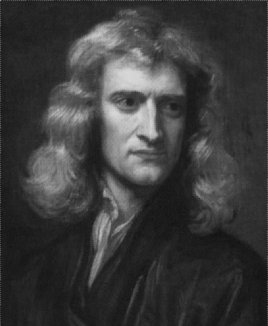
\includegraphics[width=0.25\textwidth]{figures/Newton}
  \end{flushright}
  \vspace*{-4cm}
  \begin{block}{Standard form of a nonlinear system}
    \[ \hspace*{-1cm} -\nabla \cdot \bigl(\vert\nabla u\vert^{\mathfrak{p}-2} \nabla u \bigr) - \lambda e^u = F(u) = 0 \]
  \end{block}
  
  \begin{block}{Iteration}
    \vspace*{-0.5cm}
    \begin{align*}
      \text{Solve:} & \qquad J(u) w = -F(u) \\
      \text{Update:} & \qquad u^+ \gets u + w
    \end{align*}
    \begin{itemize}
    \item Quadratically convergent near a root: $|u^{n+1}-u^*| \in \mathcal{O} \Big(|u^n-u^*|^2\Big)$
    \item Picard is the same operation with a different $J(u)$
    \end{itemize}
  \end{block}
  
  \begin{block}{Jacobian Matrix for $\mathfrak{p}$-Bratu Equation}
    \vspace*{-0.5cm}
        \begin{gather*}
         J(u) w \sim -\nabla \bigl[ (\eta {\mathbf{1}} + \eta' \nabla u \otimes \nabla u) \nabla w \bigr] - \lambda e^u w \\
          \eta' = \frac{\mathfrak{p}-2}{2} \eta / (\epsilon^2 + \gamma)
        \end{gather*}
  \end{block}
\end{frame}


\begin{frame}{SNES}
  
  \begin{block}{Scalable Nonlinear Equation Solvers}
    \begin{itemize}
     \item Newton solvers: Line Search, Thrust Region
     \item Inexact Newton-methods: Newton-Krylov
     \item Matrix-Free Methods: With iterative linear solvers
    \end{itemize}
  \end{block}
  
  \begin{block}{How to get the Jacobian Matrix?}
    \begin{itemize}
     \item Implement it by hand
     \item Let PETSc finite-difference it
     \item Use Automatic Differentiation software
    \end{itemize}
  \end{block}
\end{frame}

\begin{frame}{Nonlinear solvers in PETSc SNES}
 \begin{block}{Nonlinear solvers in PETSc SNES}
  \begin{description}
  \item[LS, TR] Newton-type with line search and trust region
  \item[NRichardson] Nonlinear Richardson, usually preconditioned
  \item[VIRS, VISS] reduced space and semi-smooth methods for variational inequalities
  \item[QN] Quasi-Newton methods like BFGS
  \item[NGMRES] Nonlinear GMRES
  \item[NCG] Nonlinear Conjugate Gradients
  \item[GS] Nonlinear Gauss-Seidel/multiplicative Schwarz sweeps
  \item[FAS] Full approximation scheme (nonlinear multigrid)
  \item[MS] Multi-stage smoothers, often used with FAS for hyperbolic problems
  \item[Shell] Your method, often used as a (nonlinear) preconditioner
  \end{description}
 \end{block}
\end{frame}


%\begin{frame}[fragile]
\frametitle{Flow Control for a PETSc Application}

\begin{center}
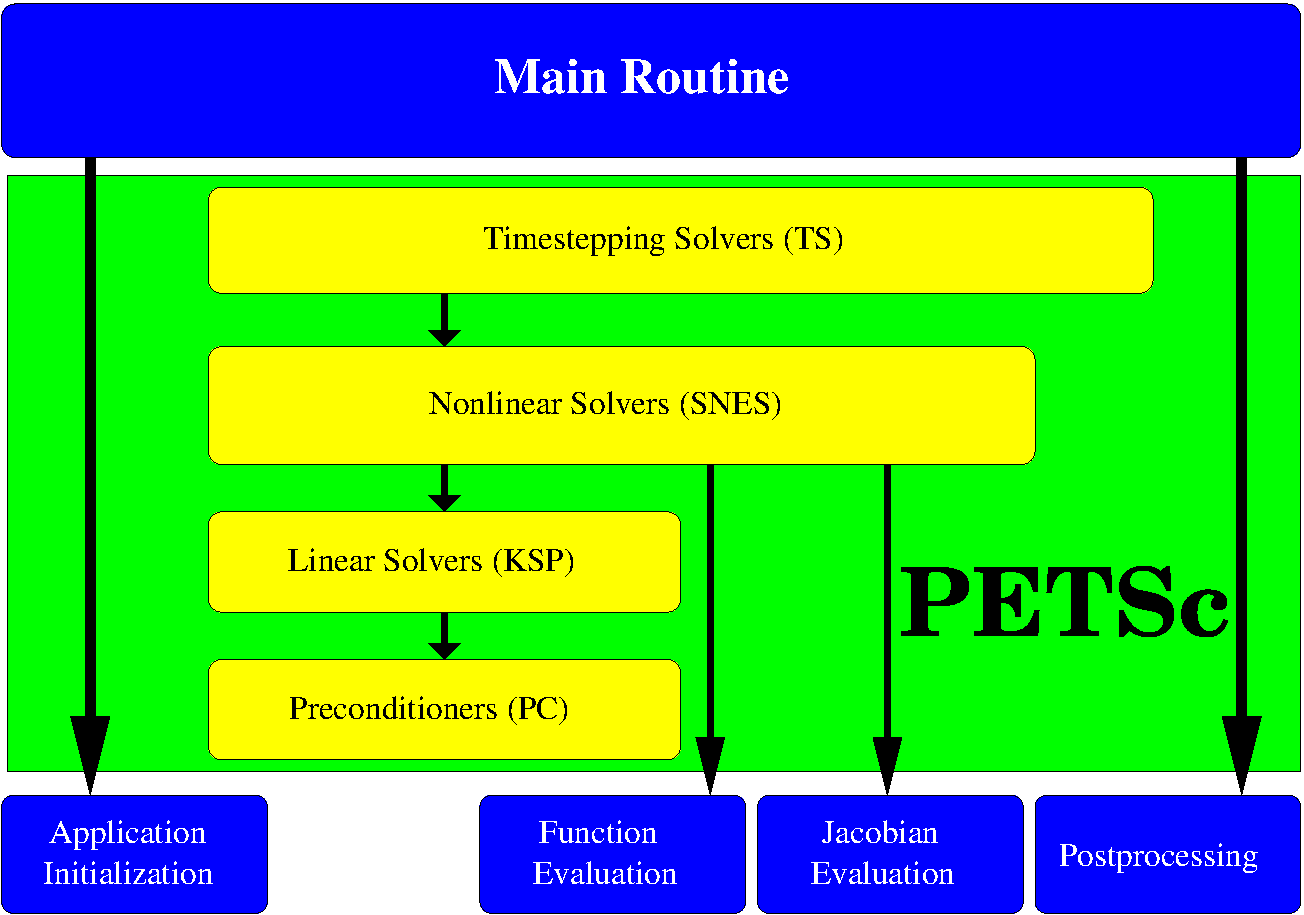
\includegraphics[width=4.0in]{figures/FlowControl}
\end{center}
\end{frame}

\begin{frame}[fragile]
\frametitle{SNES Paradigm}

\begin{block}{SNES Interface based upon Callback Functions}
\begin{itemize}
  \item \lstinline|FormFunction()|, set by \lstinline|SNESSetFunction()|
  \item \lstinline|FormJacobian()|, set by \lstinline|SNESSetJacobian()|
\end{itemize}
\end{block}
%\bigskip

 \begin{block}{Evaluating the nonlinear residual $F(x)$}
\begin{itemize}
  \item Solver calls the \textbf{user's} function

  \medskip

  \item User function gets application state through the \lstinline|ctx| variable
\end{itemize}
 \end{block}

   \begin{center}
    \color{red} PETSc \emph{never} sees application data
  \end{center}

\end{frame}

\begin{frame}[fragile]{SNES Function}

\begin{align*}
 F(u) = 0
\end{align*}

The user provided function which calculates the nonlinear residual has signature
\begin{lstlisting}
  PetscErrorCode (*func)(SNES snes,
                         Vec x,Vec r,
                         void *ctx)
\end{lstlisting}

\begin{itemize}
  \item \lstinline|x| - The current solution
  \item \lstinline|r| - The residual
  \item \lstinline|ctx| -  The user context passed to \lstinline|SNESSetFunction()|
  \begin{itemize}
    \item Use this to pass application information, e.g.~physical constants
  \end{itemize}
\end{itemize}

\end{frame}

\begin{frame}[fragile]{SNES Jacobian}

\begin{block}{User-provided function calculating the Jacobian Matrix}
\begin{lstlisting}
PetscErrorCode (*func)(SNES snes,Vec x,Mat *J,Mat *M,
                       MatStructure *flag,void *ctx)
\end{lstlisting}

\begin{itemize}
  \item \lstinline|x| - The current solution
  \item \lstinline|J| - The Jacobian
  \item \lstinline|M| -  The Jacobian preconditioning matrix (possibly J itself)
  \item \lstinline|ctx| - The user context passed to \lstinline|SNESSetFunction()|
  \begin{itemize}
    \item Use this to pass application information, e.g. physical constants
  \end{itemize}

  \item Possible \lstinline|MatStructure| values are:
  \begin{itemize}
    \item \lstinline|SAME_NONZERO_PATTERN|
    \item \lstinline|DIFFERENT_NONZERO_PATTERN|
  \end{itemize}
\end{itemize}
\end{block}

\begin{block}{Alternatives}
\begin{itemize}
  \item a builtin sparse finite difference approximation (``coloring'')
  \item automatic differentiation (ADIC/ADIFOR)
\end{itemize}
\end{block}

\end{frame}

\begin{frame}[fragile]{Finite Difference Jacobians}

\begin{block}{PETSc can compute and explicitly store a Jacobian}
 
 \begin{itemize}
  \item Dense
    \begin{itemize}
    \item Activated by \lstinline|-snes_fd|
    \item Computed by \lstinline|SNESDefaultComputeJacobian()|
    \end{itemize}
  \item Sparse via colorings
    \begin{itemize}
    \item Coloring is created by \lstinline|MatFDColoringCreate()|
    \item Computed by \lstinline|SNESDefaultComputeJacobianColor()|
    \end{itemize}
  \end{itemize}
  
\end{block}

  \begin{block}{Also Matrix-free Newton-Krylov via 1st-order FD possible}
  \begin{itemize}
  \item Activated by \lstinline|-snes_mf| without preconditioning
  \item Activated by \lstinline|-snes_mf_operator| with user-defined preconditioning
    \begin{itemize}
    \item Uses preconditioning matrix from \lstinline|SNESSetJacobian()|
    \end{itemize}
  \end{itemize}
  \end{block}

\end{frame}


\begin{frame}[fragile]{DMDA and SNES}
 
  \begin{block}{Fusing Distributed Arrays and Nonlinear Solvers}
   \begin{itemize}
    \item Make DM known to SNES solver
      \begin{lstlisting}
 SNESSetDM(snes,dm);
      \end{lstlisting}

    \item Attach residual evaluation routine
      \begin{lstlisting}
 DMDASNESSetFunctionLocal(dm,INSERT_VALUES,
        (DMDASNESFunction)FormFunctionLocal,
                          &user);
      \end{lstlisting}
   \end{itemize}
  \end{block}

  \begin{block}{Ready to Roll}
   \begin{itemize}
    \item First solver implementation completed
    \item Uses finite-differencing to obtain Jacobian Matrix
    \item Rather slow, but scalable!
   \end{itemize}
  \end{block}

 
\end{frame}






%
% GPU Summary
%
\begin{frame}{PETSc}
   \begin{center} \Large \textbf{PETSc and GPUs} \end{center}
\end{frame}




% \begin{frame}{Why bother?}
%   \begin{center} \vspace*{-0.5cm}
%    \includegraphics[width=0.9\textwidth]{figures/cuda-advantage-2}
%   \end{center}
% \end{frame}
% 
% \begin{frame}{Why bother?}
%   \begin{center} \vspace*{-0.3cm}
%    \includegraphics[width=0.6\textwidth]{figures/cuda-advantage} \\
%    \visible<2->{
%    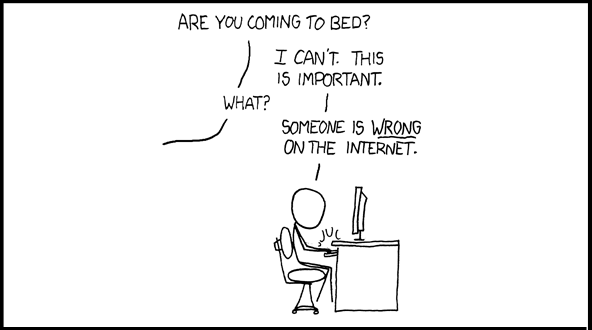
\includegraphics[width=0.6\textwidth]{figures/xkcd-someone-wrong}
%    }
%   \end{center}
% \end{frame}


\begin{frame}{Why bother?}
  \begin{center}
   \LARGE \hspace*{-1cm} \emph{Don't believe anything \\ \hspace*{1cm}unless you can run it}
  \end{center}
  \hspace*{6cm}Matt Knepley
\end{frame}



\begin{frame}{Why bother?}
  \begin{block}{GFLOPs/Watt}
  \begin{center} \vspace*{-0.5cm}
   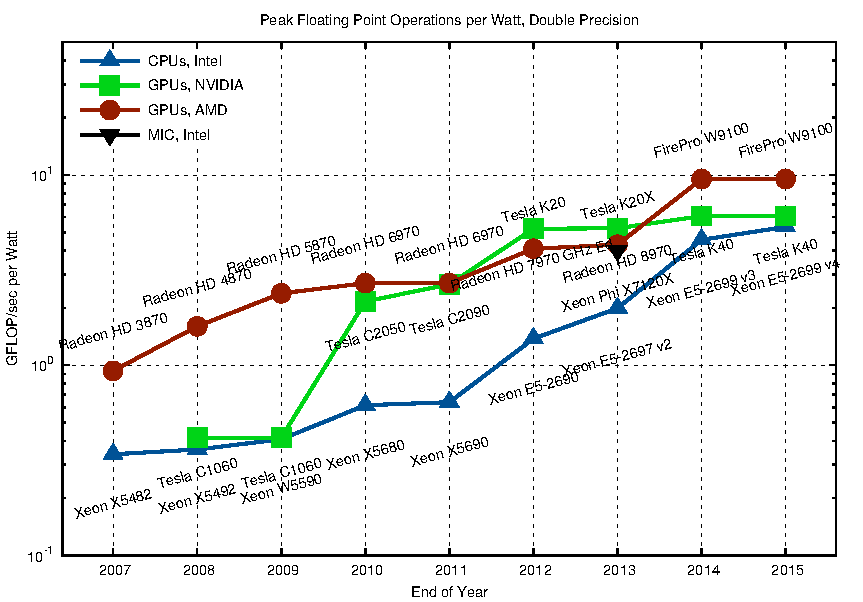
\includegraphics[width=0.95\textwidth]{figures/gflops-per-watt-dp.pdf}
  \end{center}
  \end{block}
\end{frame}



\begin{frame}{Why bother?}
  \begin{block}{Procurements}
  \begin{itemize}
   \item Theta (ANL, 2016): 2nd generation INTEL Xeon Phi
   \item Summit (ORNL, 2017), Sierra (LLNL, 2017): NVIDIA Volta GPU
   \item Aurora (ANL, 2018): 3rd generation INTEL Xeon Phi
  \end{itemize}
  \end{block}
  
  \begin{center} \vspace*{-0.5cm}
   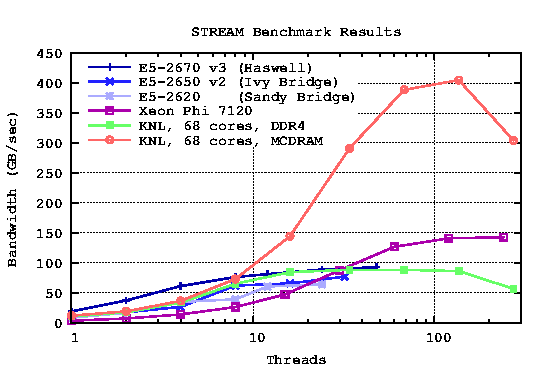
\includegraphics[width=0.75\textwidth]{figures/stream-knl.pdf} \\
   {\tiny https://www.karlrupp.net/2016/07/knights-landing-vs-knights-corner-haswell-ivy-bridge-and-sandy-bridge-stream-benchmark-results/}
  \end{center}

\end{frame}


%%%%%%%%%%%%%%%%%%%%%%%%%%%%%%%%%%%%%%%%%



\begin{frame}{Current Status}
  \begin{center}
    \Large PETSc on GPUs and MIC: \\[1em] Current Status
  \end{center}
\end{frame}

\begin{frame}[fragile]
\frametitle{Available Options}

 \begin{minipage}{0.75\textwidth}
  \begin{block}{Native on Xeon Phi}
  \begin{itemize}
   \item Cross-compile for Xeon Phi
  \end{itemize}
  \end{block}

  \begin{block}{CUDA}
  \begin{itemize}
   \item CUDA-support through CUSP as well as native
   \item \lstinline|-vec_type cusp -mat_type aijcusp|
   \item \lstinline|-vec_type cuda -mat_type aijcusparse|
   \item Only for NVIDIA GPUs
  \end{itemize}
  \end{block}

  \begin{block}{CUDA/OpenCL/OpenMP}
  \begin{itemize}
   \item CUDA/OpenCL/OpenMP-support through ViennaCL
   \item \lstinline|-vec_type viennacl -mat_type aijviennacl|
   \item OpenCL on CPUs and MIC fairly poor
  \end{itemize}
  \end{block}
 \end{minipage}
 \begin{minipage}{0.23\textwidth}
 \vspace*{1cm}
 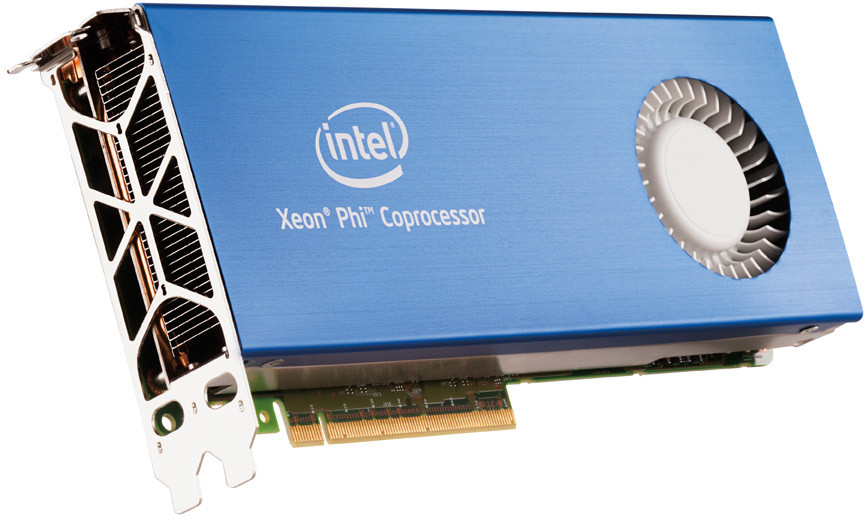
\includegraphics[width=0.99\textwidth]{figures/xeon-phi.jpg} \\[1.5em]
 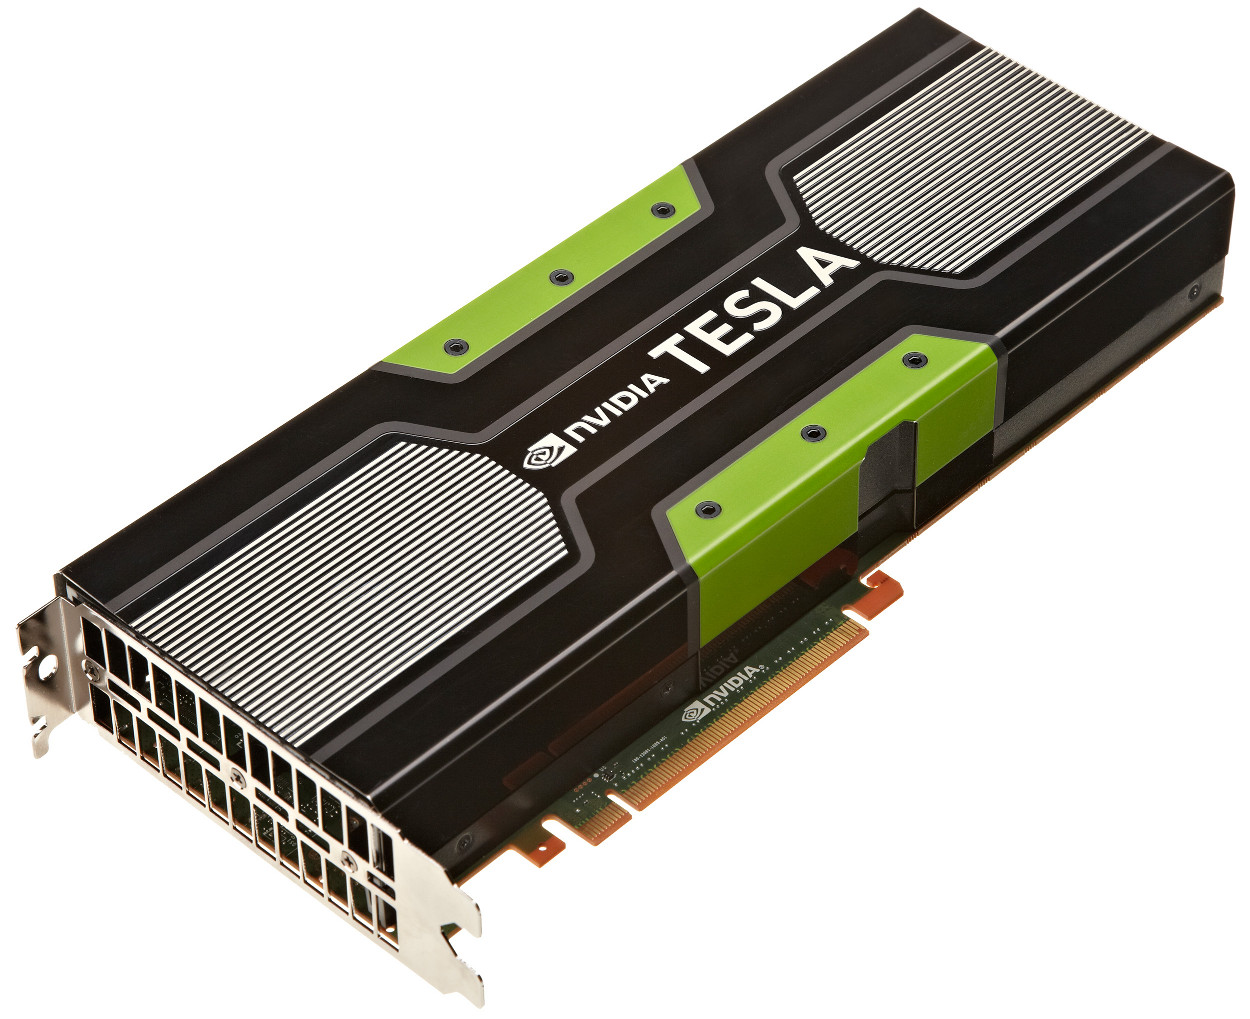
\includegraphics[width=0.99\textwidth]{figures/TeslaK20.jpg} \\[1.5em]
 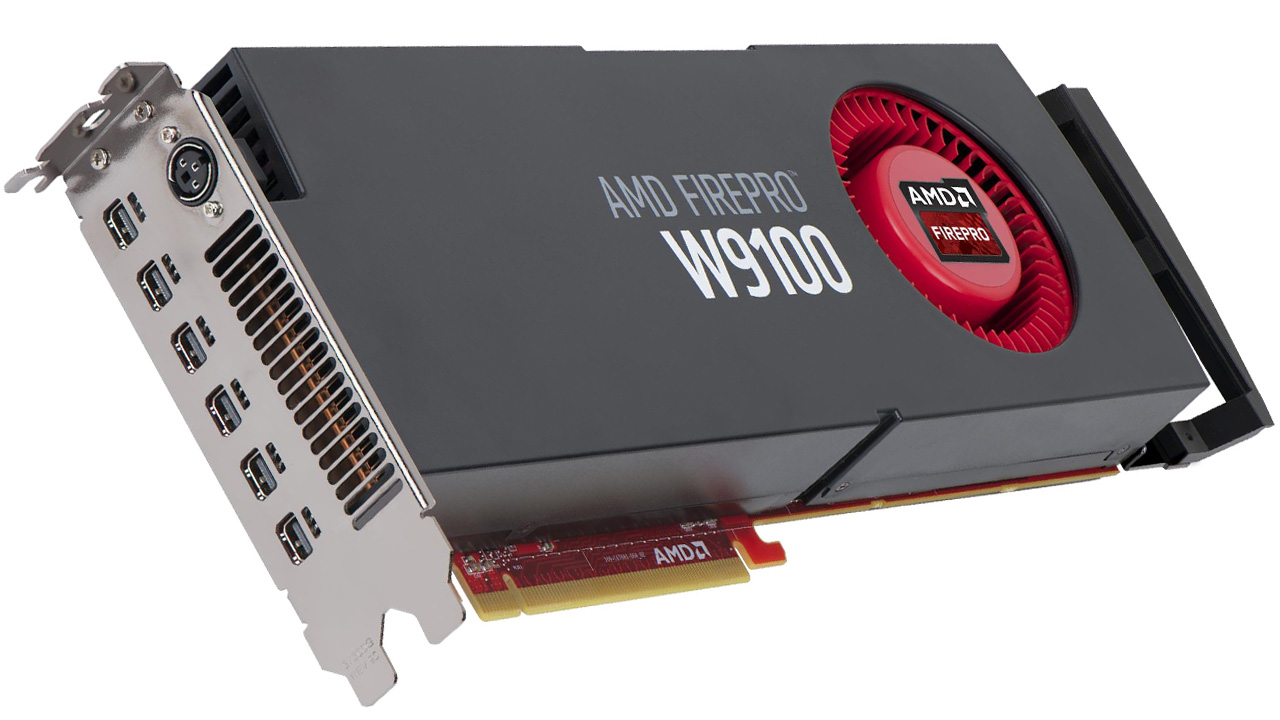
\includegraphics[width=0.99\textwidth]{figures/w9100.jpg} \\[1.5em]
 \end{minipage}


\end{frame}


% Configure PETSc
\begin{frame}[fragile]
\frametitle{Configuration}
  \begin{block}{CUDA}
    \begin{itemize}
     \item CUDA-enabled configuration (minimum)
     \begin{lstlisting}
 ./configure [..] --with-cuda=1
     \end{lstlisting}
     \item With CUSP:
     \begin{lstlisting}
   --with-cusp=1 --with-cusp-dir=/path/to/cusp
     \end{lstlisting}
     \item Customization:
     \begin{lstlisting}
   --with-cudac=/path/to/cuda/bin/nvcc
   --with-cuda-arch=sm_20
     \end{lstlisting}
    \end{itemize}
  \end{block}
  
  \begin{block}{OpenCL (ViennaCL)}
    \begin{itemize}
     \item OpenCL-enabled configuration
     \begin{lstlisting}
 ./configure [..] --download-viennacl
    --with-opencl-include=/path/to/OpenCL/include
    --with-opencl-lib=/path/to/libOpenCL.so
     \end{lstlisting}
    \end{itemize}
  \end{block}
\end{frame}


% How does it work?
\begin{frame}[fragile]
\frametitle{How Does It Work?}
  \begin{block}{Host and Device Data}
  \begin{lstlisting}
struct _p_Vec {
  ...
  void          *data;            // host buffer
  PetscCUSPFlag valid_GPU_array;  // flag
  void          *spptr;           // device buffer
};
  \end{lstlisting}
  \end{block}

  \begin{block}{Possible Flag States}
  \begin{lstlisting}
  typedef enum {PETSC_CUSP_UNALLOCATED,
                PETSC_CUSP_GPU,
                PETSC_CUSP_CPU,
                PETSC_CUSP_BOTH} PetscCUSPFlag;
  \end{lstlisting}
  \end{block}

\end{frame}

\begin{frame}[fragile]
\frametitle{How Does It Work?}

  \begin{block}{Fallback-Operations on Host}
   \begin{itemize}
    \item Data becomes valid on host (\lstinline|PETSC_CUSP_CPU|)
      \begin{lstlisting}
PetscErrorCode VecSetRandom_SeqCUSP_Private(..) {
  VecGetArray(...);
  // some operation on host memory
  VecRestoreArray(...);
}
      \end{lstlisting}
   \end{itemize}
  \end{block}

  %\pause 
  
  \begin{block}{Accelerated Operations on Device}
   \begin{itemize}
    \item Data becomes valid on device (\lstinline|PETSC_CUSP_GPU|)
      \begin{lstlisting}
PetscErrorCode VecAYPX_SeqCUSP(..) {
  VecCUSPGetArrayReadWrite(...);
  // some operation on raw handles on device
  VecCUSPRestoreArrayReadWrite(...);
}
      \end{lstlisting}
   \end{itemize}
  \end{block}

\end{frame}


% Example with ILU
\begin{frame}[fragile]
\frametitle{Example}
  \begin{block}{KSP ex12 on Host}
  \begin{itemize}
   \item
    \begin{lstlisting}
$> ./ex12
    -pc_type ilu -m 200 -n 200 -log_summary
    \end{lstlisting}
    \begin{lstlisting}
KSPGMRESOrthog       228 1.0 6.2901e-01
KSPSolve               1 1.0 2.7332e+00
    \end{lstlisting}

  \end{itemize}
  \end{block}

  %\pause
  
  \begin{block}{KSP ex12 on Device}
  \begin{itemize}
   \item
    \begin{lstlisting}
$> ./ex12 -vec_type cusp -mat_type aijcusp
    -pc_type ilu -m 200 -n 200 -log_summary
    \end{lstlisting}
    \begin{lstlisting}
[0]PETSC ERROR: MatSolverPackage petsc does not support matrix type seqaijcusp
    \end{lstlisting}

  \end{itemize}
  \end{block}
  \vspace*{0.4cm}

\end{frame}


% Example without preconditioner
\begin{frame}[fragile]
\frametitle{Example}
  \begin{block}{KSP ex12 on Host}
  \begin{itemize}
   \item
    \begin{lstlisting}
$> ./ex12 
    -pc_type none -m 200 -n 200 -log_summary
    \end{lstlisting}
    \begin{lstlisting}
KSPGMRESOrthog      1630 1.0 4.5866e+00
KSPSolve               1 1.0 1.6361e+01
    \end{lstlisting}

  \end{itemize}
  \end{block}

  %\pause
  
  \begin{block}{KSP ex12 on Device}
  \begin{itemize}
   \item
    \begin{lstlisting}
$> ./ex12 -vec_type cusp -mat_type aijcusp
    -pc_type none -m 200 -n 200 -log_summary
    \end{lstlisting}
    \begin{lstlisting}
MatCUSPCopyTo          1 1.0 5.6108e-02
KSPGMRESOrthog      1630 1.0 5.5989e-01
KSPSolve               1 1.0 1.0202e+00
    \end{lstlisting}

  \end{itemize}
  \end{block}

\end{frame}


% Pitfalls
\begin{frame}[fragile]
\frametitle{Pitfalls}
  \begin{block}{Pitfall: Repeated Host-Device Copies}
  \begin{itemize}
   \item PCI-Express transfers kill performance
   \item Complete algorithm needs to run on device
   \item Problematic for explicit time-stepping, etc.
  \end{itemize}
  \end{block}

  %\pause
  
  \begin{block}{Pitfall: Wrong Data Sizes}
  \begin{itemize}
   \item Data too small: Kernel launch latencies dominate
   \item Data too big: Out of memory
  \end{itemize}
  \end{block}

  %\pause
  
  \begin{block}{Pitfall: Function Pointers}
  \begin{itemize}
   \item Pass CUDA function ``pointers'' through library boundaries?
   \item OpenCL: Pass kernel sources, user-data hard to pass
   \item Composability?
  \end{itemize}
  \end{block}

\end{frame}


% Overview of what is available
\begin{frame}[fragile]
\frametitle{Current GPU-Functionality in PETSc}
  
  \begin{block}{Current GPU-Functionality in PETSc}
  \begin{center}
  \renewcommand{\arraystretch}{1.2}
  \begin{tabular}{|l|c|c|}
   \hline
                     & \textbf{CUSP/CUDA}  & \textbf{ViennaCL} \\
   \hline
   Programming Model & CUDA  & CUDA/OpenCL/OpenMP \\
   \hline
   Operations        & Vector, MatMult & Vector, MatMult \\
   \hline
   Matrix Formats    & CSR, ELL, HYB  & CSR \\
   \hline
   Preconditioners   & SA-AMG, BiCGStab & - \\
   \hline
   MPI-related       & Scatter & - \\
   \hline
  \end{tabular}
  \end{center}
  \end{block}

  \begin{block}{Additional Functionality}
   \begin{itemize}
    \item MatMult via cuSPARSE
    \item OpenCL residual evaluation for PetscFE
   \end{itemize}
  \end{block}


\end{frame}






\begin{frame}{Current Directions}
  \begin{center}
    \Large PETSc on GPUs and MIC: \\[1em] Current Directions \\[1em]
  \end{center}
\end{frame}


% cuBLAS and friends
\begin{frame}[fragile]
\frametitle{Current: CUDA}
  \begin{block}{Split CUDA-buffers from CUSP}
  \begin{itemize}
   \item Vector operations by cuBLAS
   \item MatMult by different packages
   \item CUSP (and others) provides add-on functionality
  \end{itemize}
  \end{block}
  
  %\pause 
  \begin{block}{More CUSP Functionality in PETSc}
   \begin{itemize}
    \item Relaxations (Gauss-Seidel, SOR)
    \item Polynomial preconditioners
    \item Approximate inverses
   \end{itemize}
  \end{block}

\end{frame}


% ViennaCL: CUDA, OpenCL, OpenMP
\begin{frame}[fragile]
\frametitle{Current: PETSc + ViennaCL}

\begin{minipage}{0.58\textwidth}
  \begin{block}{ViennaCL}
  \begin{itemize}
   \item CUDA, OpenCL, OpenMP backends
   \item Backend switch at \textbf{runtime}
   \item CUDA, OpenCL and OpenMP exposed in PETSc
   \item Focus on shared memory machines
  \end{itemize}
  \end{block}
\end{minipage}
\begin{minipage}{0.4\textwidth}
   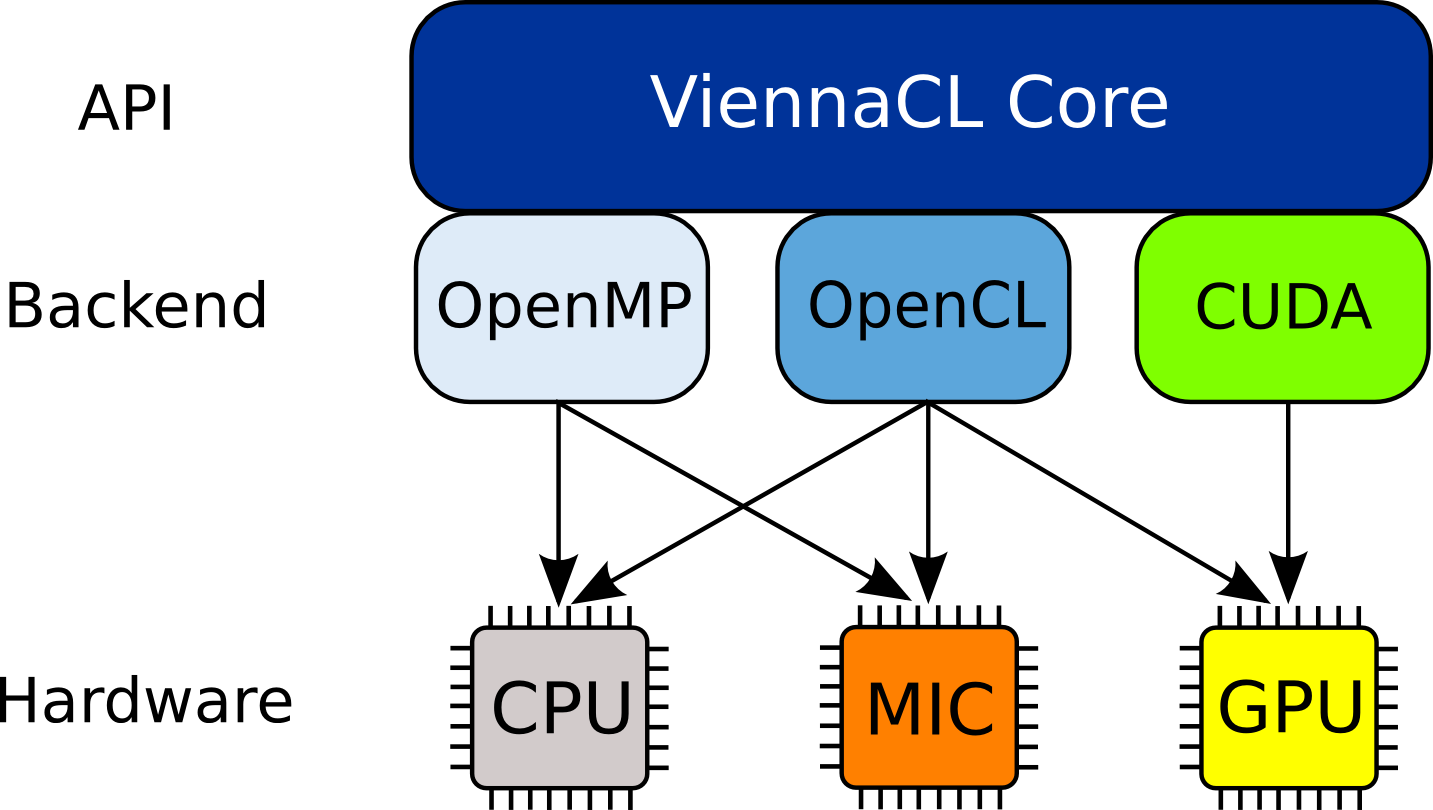
\includegraphics[width=0.999\textwidth]{figures/ViennaCL-arch}
\end{minipage}

  %\pause
  \vspace*{0.3cm}
  \begin{block}{Recent Advances}
  \begin{itemize}
   \item Pipelined Krylov solvers
   \item Fast sparse matrix-vector products
   \item Fast sparse matrix-matrix products
   \item Fine-grained algebraic multigrid
   \item Fine-grained parallel ILU
  \end{itemize}
  \end{block}

\end{frame}


\begin{frame}[fragile]
\frametitle{Current: PETSc + ViennaCL}

  \begin{block}{Current Use of ViennaCL in PETSc}
  \begin{itemize}
   \item 
  \begin{lstlisting}
 $> ./ex12 -vec_type viennacl -mat_type aijviennacl ...
  \end{lstlisting}
   \item Executes on OpenCL device
  \end{itemize}
  \end{block}

  %\pause
  
  \begin{block}{New Use of ViennaCL in PETSc}
  \begin{itemize}
   \item 
  \begin{lstlisting}
 $> ./ex12 -vec_type viennacl -mat_type aijviennacl
           -viennacl_backend openmp ...
  \end{lstlisting}
  \end{itemize}
  \end{block}

  %\pause
  
  \begin{block}{Pros and Cons}
  \begin{itemize}
   \item Use CPU + GPU simultaneously
   %\item Good PETSc performance on Theta, Aurora, Summit, ...
   \item Non-intrusive, use plugin-mechanism
   \item Non-optimal in strong-scaling limit
   \item Gather experiences for best long-term solution
  \end{itemize}
  \end{block}

\end{frame}





\begin{frame}{GPU Summary and Conclusion}

  \begin{block}{Currently Available}
    \begin{itemize}
     \item CUSP for CUDA, ViennaCL for OpenCL
     \item Automatic use for vector operations and SpMV
     \item Smoothed Agg. AMG via CUSP
      \item ViennaCL as CUDA/OpenCL/OpenMP-hydra
    \end{itemize}
  \end{block}

  \begin{minipage}{0.7\textwidth}
    \begin{block}{Current Activities}
      \begin{itemize}
      \item Use of cuBLAS and cuSPARSE
      \item Better support for $n>1$ processes
      %\item CUSolver for sparse direct solution?
      \end{itemize}
    \end{block}
  \end{minipage}
  \begin{minipage}{0.29\textwidth}
    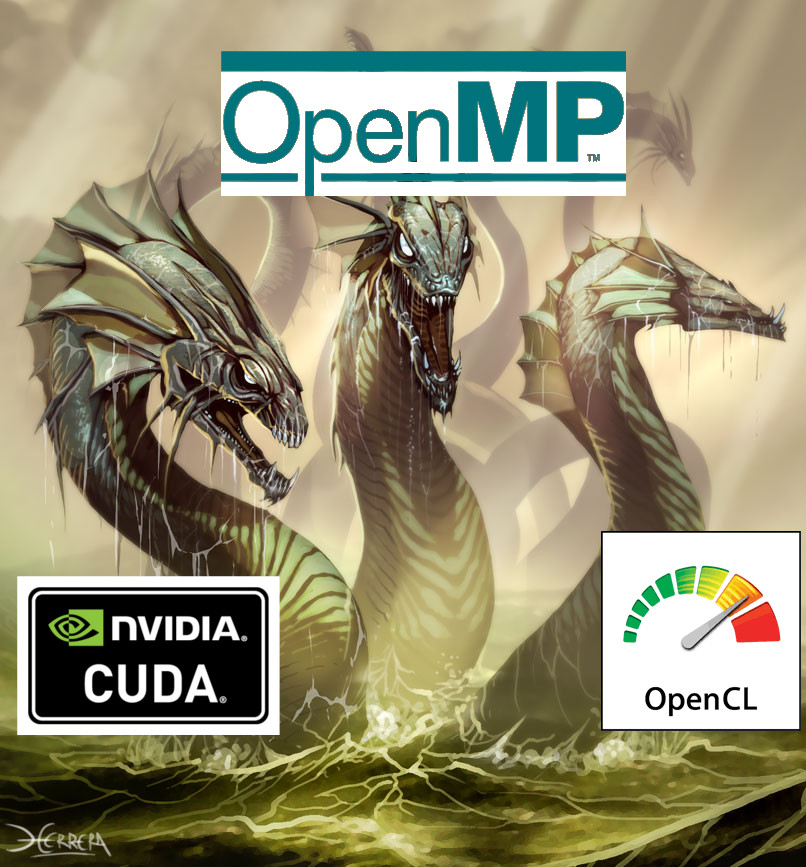
\includegraphics[width=0.99\textwidth]{figures/hydra}
  \end{minipage}

\end{frame}


%%%% Conclusion




%
% Conclusion and Wrap-Up
%
\section{Conclusions}
\begin{frame}{Conclusions}
 
 \begin{block}{PETSc can help You}
  \begin{itemize}
   \item solve algebraic and DAE problems in your application area
   \item rapidly develop efficient parallel code, can start from examples
   \item develop new solution methods and data structures
   \item debug and analyze performance
   \item advice on software design, solution algorithms, and performance
   \item \centering \texttt{petsc-\{users,dev,maint\}@mcs.anl.gov}

  \end{itemize}
 \end{block}

 \begin{block}{You can help PETSc}
  \begin{itemize}
   \item report bugs and inconsistencies, or if you think there is a better way
   \item tell us if the documentation is inconsistent or unclear
   \item consider developing new algebraic methods as plugins, contribute if your idea works
  \end{itemize}
 \end{block}

\end{frame}


